51.
\begin{figure}[ht!]
\center{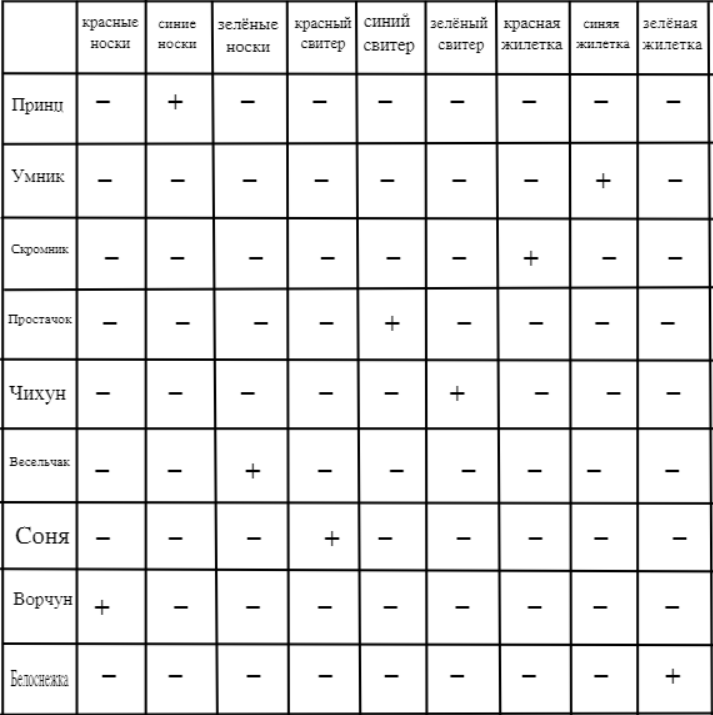
\includegraphics[scale=0.7]{pod.png}}
\end{figure}\\
Для решения этой задачи необходимо нарисовать таблицу и последовательно её заполнить. Принцу ставим $-$ во все клетки, кроме ЗЖ и СН. Умнику ставим $-$ во все клетки, кроме СН и СС. Скромнику ставим $-$ во все клетки, кроме КЖ, СС и СЖ. Простачку ставим $-$ во все клетки, кроме СС и СЖ. Чихуну и Весельчаку ставим $-$ в клетки КН, КС и КЖ. Соне ставим $-$ в КН. Весельчаку также ставим $-$ в СС и СЖ. Белоснежке ставим $+$ в ЗЖ, всем остальным в эту клетку $-$. Красные носки не могут достаться никому, кроме Ворчуна, ставим ему $+$ в эту клетку и $-$ в остальные. Зелёная жилетка досталась Белоснежке. поэтому Принц получил синие носки, ставим ему в эту клетку $+,$ всем остальным $-.$ Умнику остаётся только синяя жилетка, ставим ему в эту клетку $+,$ а всем остальным $-.$ Скромнику остаётся красная жилетка, ставим ему $+,$ а Соне $-.$ Простачку остаётся синий свитер, ставим ему $+,$ а остальным $-.$ Весельчаку остаются только зелёные носки, тогда Чихун должен получить зелёный свитер. Тогда Соне остаётся красный свитер и на этом распределение подарков окончено.\\
